Geomorfologie je věda zabývající se tvary zemského reliéfu, jeho historií a procesy, které ho utvářejí. Geneze reliéfu je komplexní proces, proto geomorfologie využívá a spojuje poznatky z celé řady dalších vědeckých disciplín (viz tab. \ref{tab:geom_a_dalsi}, obr. \ref{fig:diagramgeomorf}). Jedná se tedy o vědu syntetickou. Pojem geomorfologie vznikl spojením tří řeckých slov: geo (země), -morphos (tvar, forma) a -ology (studium).

\emph{Objektem studia} geomorfologie je zemský reliéf -- \emph{georeliéf}. Reliéf sám o sobě není hmotný, jedná se o svrchní plochu zemské kůry, která tvoří rozhraní mezi litosférou a dalšími sférami Země jako je například atmosféra či hydrosféra. Hmotným nositelem reliéfu jsou horniny zemské kůry a je jedno, jestli se jedná o pevné horniny či nezpevněné sedimenty. Georeliéf můžeme chápat i jako soubor tvarů zemského povrchu.

\begin{figure*}[h]
	\centering
	\includegraphics[width=\linewidth]{obrazky/uvod/diagram_geomorf}
	\caption{Georeliéf tvoří rozhraní mezi litosférou nebo pedosférou na jedné straně a atmosférou, hydrosférou, biosférou a antroposférou. Georeliéf ovlivňuje okolní sféry a naopak je sám jimi ovlivňován.}
	\label{fig:diagramgeomorf}
\end{figure*}


\begin{table*}[h]
	\begin{tabularx}{1\textwidth}{@{}lXX@{}}
		\toprule
		Disciplína   & Příklad přínosu pro geomorfologii                                         & Příklad přínosu z geomorfologie                                    \\ \midrule
		Geofyzika    & Mechanismus a rychlost výzdvihu                                           & Erozivní odpověď krajiny na výzdvih                                \\
		Sedimentologie &
		Rekonstrukce minulých erozních událostí ze sedimentárních záznamů &
		Podoba říčních koryt při interpretaci fluviálních sedimentů \\
		Geochemie    & Rychlost a charakter chemických reakcí při zvětrávání                     & Mobilizace prvků při zemském povrchu                               \\
		Hydrologie   & Četnost a intenzita zápav                                                 & Koncentrace sedimentů ve vodních tocích                            \\
		Klimatologie & vliv klimatických prvků na rychlost a charakter geomorfologických procesů & Vliv reliéfu na klimatické prvky                                   \\
		Pedologie    & Vliv půdních vlastností na stabilitu svahu                                & Vliv reliéfu na pedogenetické procesy                              \\
		Biologie     & Role vegetace jako ochrany před erozí                                     & Vliv reliéfu na stanovištní podmínky                               \\
		Inženýrství  & Nástroje pro analýzu stability svahu                                      & Identifikace morfologických prvků ukazujících na nestabilitu svahu \\
		Věda o vesmíru &
		Kontext pro pochopení zvláštních vlastností prostředí, které vytváří reliéf na Zemi &
		Interpretace planetárních krajin na základě analogie s pozemskými formami reliéfu \\ \bottomrule
	\end{tabularx}
	\caption{Příklady vztahu mezi geomorfologií a spřízněnými disciplínami (upraveno podle \textcite{summerfieldGlobalGeomorphologyIntroduction1999})}
	\label{tab:geom_a_dalsi}
\end{table*}


\emph{Předmětem geomorfologie} je vznik jednotlivých forem reliéfu neboli \emph{morfogeneze}, kdy a jak rychle vznikaly \emph{morfochronologie}, jaké mají (geo)metrické vlastnosti -- \emph{morfometrie}. Geomorfologa zajímají ale také současné reliéfotvorné procesy -- \emph{morfodynamika} či vztahy mezi jednotlivými formami georeliéfu a dalšími složkami krajiny a také jejich prostorové rozmístění (\emph{morfogeografie}).

\section{Proč se zabývat geomorfologií?}
Povrch Země je dynamický, mění se v čase a prostoru. Jeho vývoj je ovlivněn celou řadou faktorů, člověka nevyjímaje. Geomorfologické procesy jsou často významným \emph{geohazardem}. Sesuvy, povodně, větrné bouře každý rok způsobůjí rozsáhlé škody a mají na svědomí množství lidských životů. Nejde ale jen o přírodní hazardy. Znalosti geomorfologie jsou důležité pro jakékoliv plánování v krajině, krajinný management. Bez znalosti možných úskalí, problematických faktorů, různých limit území nelze kvalitně a s rozumem v krajině hospodařit. Špatným plánováním, nevhodnou lokalizací staveb je můžete vystavit zbytečnému riziku (sesuvy, povodně, skalní řícení) a ohrozit tak i jejich obyvatele. 
%Nevhodným hospodařením na polích můžeme zesílit půdní erozi, což vede ke snižování úrodnosti pole, ale také se to může projevit i tím, že pravidelně po prudších deštích půda 
A netýká se to jen na první pohled zjevných rizik. Některé události mají tak malou frekvenci opakování, že ani nemohou být zaznamenané v jakýchkoliv lidských kronikách. Komplexním geomorfologickým výzkumem je ale možné odhalit celou řadu na první pohled skrytých nebezpečí.



\section{Stručný exkurz do historie geomorfologie}
Prvotní úvahy o vývoji reliéfu lze najít už v období antiky. Herodotus (484 př. n. l. -- 430 př. n. l.) popsal vývoj Nilské delty a spočítal její stáří na základě rychlosti ukládání sedimentů. Aristoteles například uvažoval o střídání pevnin a moří. Tam, kde kdysi bylo moře je v současnosti souš a naopak. Lucius Annaeus Seneca přemýšlel o síle vodních toků a jejich erozní činnosti. Stejným tématem se zabýval v 15. století i Leonardo da Vinci.

Základní geomrofologické koncepty byly položeny až ke konci 18. století. V roce 1785 představil James Hutton svou představu, že zemský povrch je dominantně formován postupnou vodní erozí a ne katastrofickými událostmi. Na Huttonových základech stavěl Charles Lyell, který v práci \textit{Principles of Geology} vypracoval myšlenky \emph{uniformitarianismu} (označované taky jako \emph{princip uniformity}, \emph{aktualismus}), který má čtyři základní principy:
\begin{enumerate}
	\item \emph{Jednota zákonů:} přírodní zákony jsou konstantní v čase a prostoru.
	\item \emph{Jednota procesů:} pokud lze vysvětlit události dob minulých procesy, které známe ze současnosti, není třeba vymýšlet další neznámé vysvětlení.
	\item \emph{Jednota rychlosti:} změny na zemském povrchu jsou pomalé, ustálené a postupné. Velké katastrofické události (povodně, zemětřesení) mají jen omezený prostorový dosah a v minulosti se děly se stejnou frekvencí jako je tomu v současnosti.
	\item \emph{Jednota stavu:} Země vždy vypadala a chovala se stejně jako v minulosti.
\end{enumerate}

Oproti aktualismu stály myšlenky \emph{katastrofismu}, tedy že velká část forem reliéfu je vytvořená rychlými, katastrofickými událostmi a ne pomalým, dlouhodobým vývojem. 
%
%Louis Agassiz (1807--1873)
%
%Grove Karl Gilbert (1843--1918)

W. M. Davis (1850--1934) (Obr. \ref{fig:davies}) formuloval jeden z prvních modelů vývoje georeliéfu. Jedná se o geografický (Davisův) \emph{cyklus eroze}. Dle jeho teorie je georeliéf funkcí tří veličin: geologické stavby (struktury), procesu a času. 
\begin{figure}[h]
	\centering
	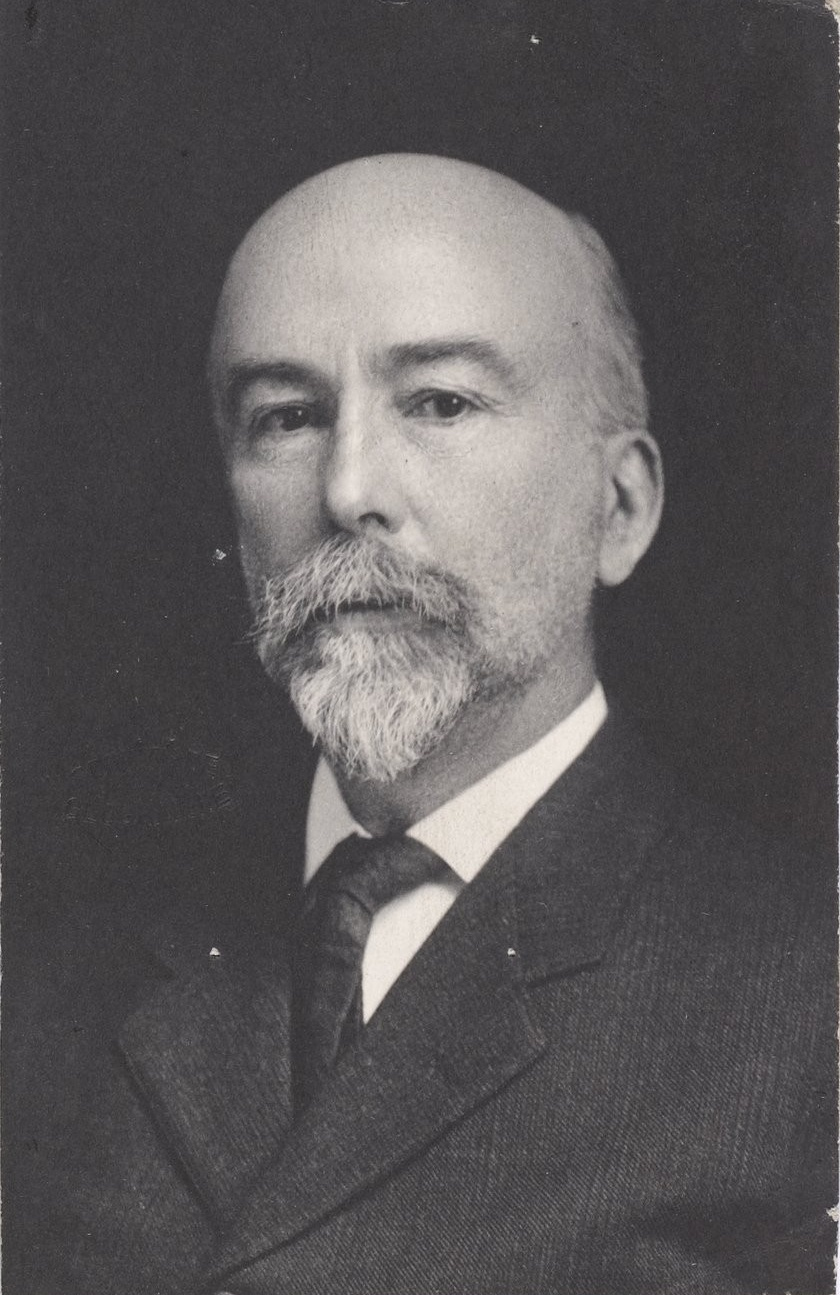
\includegraphics[width=0.7\linewidth]{obrazky/uvod/davies}
	\caption{William Morris Davies (zdroj: Bibliothèque nationale de France https://gallica.bnf.fr/ark:/12148/btv1b8453640z, volné dílo)}
	\label{fig:davies}
\end{figure}

Proti představám W. M. Davise vystupoval Walther Penck, který odmítal představu, že po rychlém výzdvihu může být dlouhé stabilní období pro vývoj následných forem reliéfu. V jeho představách je podoba krajiny závislá na tom, zda výzdvih se zvětšuje, snižuje nebo je konstantní v průběhu času.
Obecně můžeme říct, že v počátcích byla evropská goemorfologie do velké míry popisná a klasifikační, kdežto americká byla vysvětlující -- interpretační.

Od konce 40. ket dochází zejména v USA a UK k rozvoji kvantitativní geomorfologie. Průkopníkem je R.E. Horton, který v roce 1945 publikoval práci o hydrologii povodí. Následující roky se tak rozvíjela geomorfometrie a intenzivně se měřily geomorfologické procesy v terénu. V kontinentální Evropě se během té doby intenzivněji rozvíjela klimatická geomorfologie.

Během 60. a 70. let se geomorfologie v UK a USA přeorientovala na tvorbu prediktivních modelů k předpovídání krátkodobých změn reliéfu. Postupně narůstala globalizace geomorfologie až do současné podoby.
%\section{Česká a československá geomorfologie}
%\todo[inline]{dopsat}

\section{Geomorfologické disciplíny}
Geomorfologii můžeme rozdělit podrobněji podle předmětu studia do několika disciplín.
\begin{enumerate}
	\item \emph{Strukturní geomorfologie} se zabývá vlivem geologické struktury na tvary zemského povrchu.
	\item \emph{Klimatická geomorfologie} studuje vliv klimatu na vývoj reliéfu.
	\item \emph{Dynamická geomorfologie} zkoumá geomorfologické procesy.
	\item \emph{Paleogeomorfologie} nebo také historická geomorfologie se zabývá výzkumem georeliéfu minulých geologických období.
	\item \emph{Antropogenní geomorfologie} studuje tvary reliéfu, které člověk vytváří a procesy, které způsobují jejich vznika a vývoj. Také sleduje jak člověk ovlivňuje přírodní morfogenetické procesy.
	\item \emph{Aplikovaná geomorfologie} neboli užitá geomorfologie aplikuje geomorfologické poznatky a přístupy pro řešení celé řady socioekonomických problémů.
\end{enumerate}
